\chapter{DISCUSSION \& ANALYSIS}
\section{Introduction}
After clarifying the data collection process and the relevant procedures adopted for
the analysis, this chapter aims to examine the previously collected data in order to determine
the definitive truth regarding hressing AI into higher education. To this end, statistical
tables and graphs would be disclosed. The findings of this
paper are consistent with previous research results on the practical ways of implementing AI into
humanities, students' point of view about their preformance while using AI, challanges and oppurtunites.
In short, the survey’s results indicate that students academic performance is improved while using AI.
\section{Results}
% In this sections, a descriptive statistic technique was used to
% interpret the data collected from English
% university students through filling out Google form.
The data collected from the survey conducted among English university students 
revealed compelling insights into the students' perceptions and experiences with AI-driven tools. 
The analysis utilized descriptive statistical techniques to interpret the responses gathered through the questionnaire.
The questionnair divided into two main parts: the first part is to investigate
whether the students' academic performance have improved or not while using AI-driven. The second
part is about challenges and oportunites faced during using AI for academic studies.

\subsection{the students' academic performance while using AI-driven tools}
\begin{figure}[h]
	\centering
	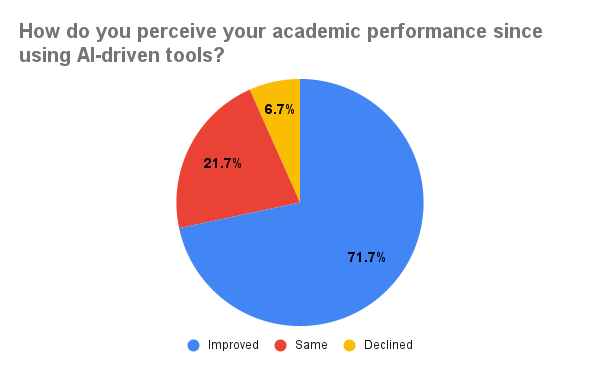
\includegraphics[width=11cm, height=7cm]{./chap4/figures/prf}
	\captionof{figure}{perceive academic performance using AI-driven tools}
\end{figure}
After assessing the respondents’ opinions on the use of AI-driven tools
and students' academic preformance, it is obvious that the majority
of their academic preformance was improved. it is clearly shown that
74.3\% agreed that AI improve their academic performance. In addition to
20\% of respondents believed that the use of AI didn't affect their academic
performance. Whereas 4.7\% showed their negative resulte believing that AI
affect their academic preformance to be declined while using it.

\subsection{Challenges and opportunites faced while using AI-driven tools in academic setting}

\begin{figure}[H]
	\centering
	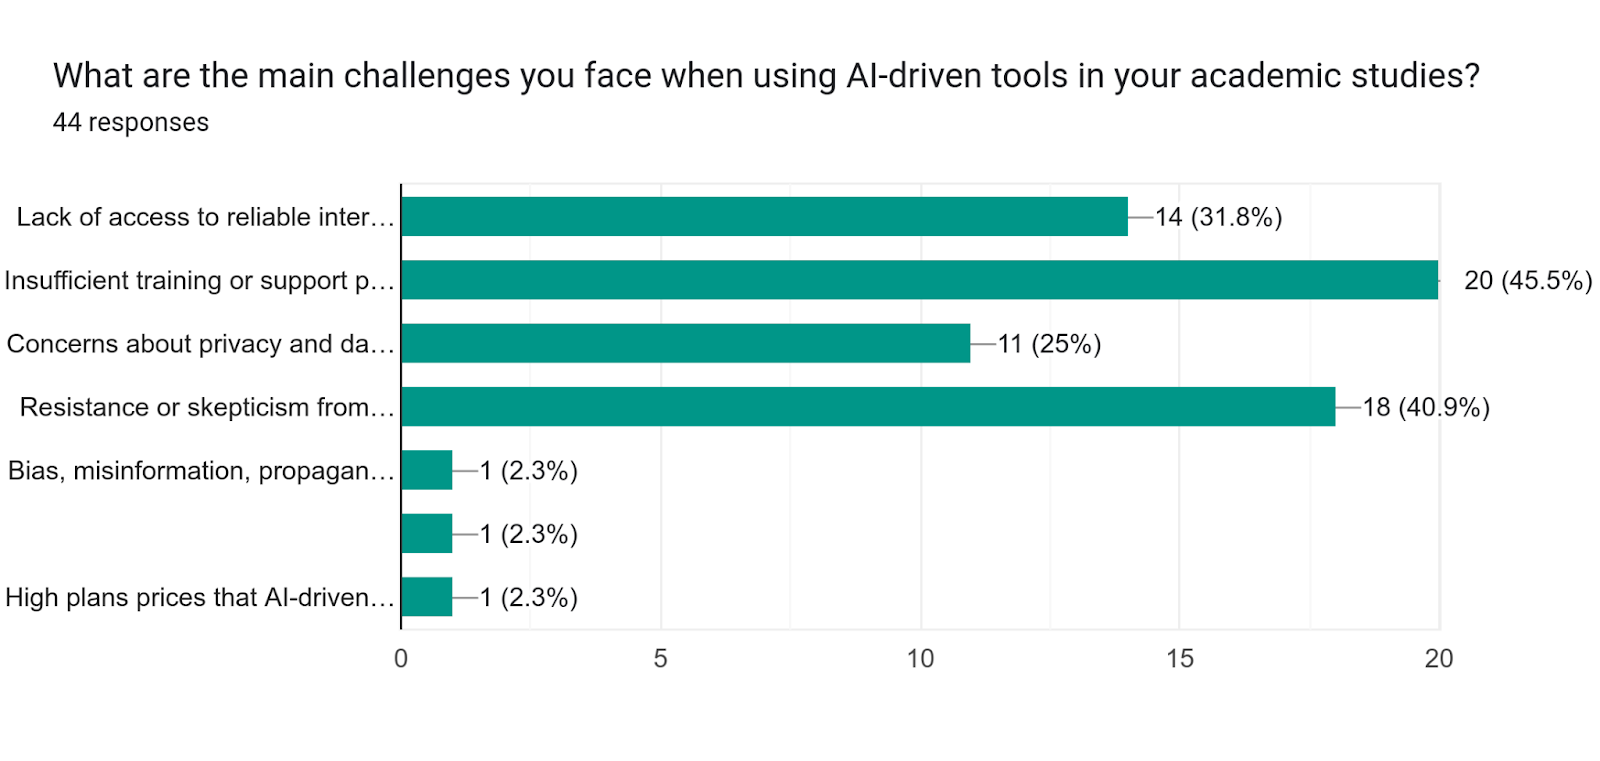
\includegraphics[width=17cm, height=9cm]{./chap4/figures/chall}
	\captionof{figure}{challenges faced when using AI-driven tools in academic setting}
\end{figure}

The bar chart shows the results of a survey on the challenges students
face when using AI-driven tools in their academic studies. Out of 44 respondents,
the biggest challenge was reported to be insufficient trainging for the
tools, with 45.5\% of students selecting this options. While resistance or skepticism
from professors towards using AI-driven tools was reported to be the second challenge
face by students with 40.9\%.
Following this was lack of access to reliable internet, with 31.8\% of students
reporting this as a challenge.
A smaller percentage of students reported facing challenges with pricacy and data security matters
with 25\%. while 2.3\% was bias, misinformation, propaganda in the AI tools and high prices of the AI-driven tools.

% The blow bar chart has shown that 45.5\% of English university
% students face Insufficient training
% as main challenge. In addition 40.9\% was resistance
% or skepticism from professors towards using AI-driven tools in
% academic settings. While 31.8\% and
% 25\% were lack of access to relaible internet and privacy comcerns. whereas
% 2.3\% was bais and high plans prices that AI-driven tools offer.
